% llm-integration.tex
% Section 6: How to Integrate LLMs in the Curriculum

%%%%%%%%%%%%%%%%%%%%
\section{Integrating LLMs in the Curriculum}
%%%%%%%%%%%%%%%%%%%%

%%%%%%%%%%%%%%%%%%%%
\begin{frame}{Responsible LLM Integration}
  \begin{center}
    \textbf{LLMs are tools, not replacements for learning.}
  \end{center}
  
  \vspace{0.3cm}
  
  \begin{columns}[T]
    \begin{column}{0.48\textwidth}
      \textbf{\teal{Effective Uses:}}
      \begin{itemize}
        \item Code explanation
        \item Debugging assistance
        \item Example generation
        \item Documentation lookup
        \item Boilerplate generation
      \end{itemize}
    \end{column}
    \begin{column}{0.48\textwidth}
      \textbf{\red{Risky Uses:}}
      \begin{itemize}
        \item Blind copy-paste
        \item Security-critical code
        \item Undefined behavior analysis
        \item Performance optimization
        \item Architecture decisions
      \end{itemize}
    \end{column}
  \end{columns}
  
  \vspace{0.3cm}
  
  \begin{block}{Key Principle}
    Teach students to \textit{verify} LLM output, not \textit{trust} it blindly.
  \end{block}
  
  % Speaker note: Students must develop critical evaluation skills
\end{frame}
%%%%%%%%%%%%%%%%%%%%

%%%%%%%%%%%%%%%%%%%%
\begin{frame}[fragile]{LLM-Based Debugging and Code Review}
  \begin{columns}[T]
    \begin{column}{0.48\textwidth}
      \textbf{Debugging Exercise:}
      \begin{block}{Student Code with Bug}
\begin{verbatim}
int *create_array(int n) {
  int arr[n];
  for (int i = 0; i < n; i++)
    arr[i] = i;
  return arr;  // UB!
}
\end{verbatim}
      \end{block}
      
      Ask LLM: ``What's wrong?'' \\
      Then: ``\textit{Why} is this UB?'' \\
      Verify against C standard.
    \end{column}
    \begin{column}{0.48\textwidth}
      \textbf{Code Review Workflow:}
      \begin{enumerate}
        \item Student writes code
        \item Ask LLM for feedback
        \item Critically evaluate suggestions
        \item Instructor verifies
      \end{enumerate}
      
      \textbf{Good Prompts:}
      \begin{itemize}
        \item ``Are there memory leaks?''
        \item ``Is this thread-safe?''
        \item ``Which C rule applies?''
      \end{itemize}
    \end{column}
  \end{columns}
  
  \textbf{Goal:} Use LLMs as starting points, not answers.
  
  % Speaker note: LLMs are good at pattern matching known bugs
\end{frame}
%%%%%%%%%%%%%%%%%%%%

%%%%%%%%%%%%%%%%%%%%
\begin{frame}{Assignment and Exam Design for the LLM Era}
  \begin{columns}[T]
    \begin{column}{0.48\textwidth}
      \textbf{\red{Outdated Assignments:}}
      \begin{itemize}
        \item ``Implement linked list''
        \item ``Write a sorting algorithm''
        \item ``Create a file reader''
      \end{itemize}
      
      \textit{LLMs generate these trivially.}
      
      \vspace{0.3cm}
      
      \textbf{\teal{Modern Assignments:}}
      \begin{itemize}
        \item ``Explain why this has UB''
        \item ``Optimize and measure''
        \item ``Design an API''
        \item ``Review LLM-generated code''
      \end{itemize}
    \end{column}
    \begin{column}{0.48\textwidth}
      \textbf{Exam Questions:}
      
      \textbf{Semantics:}
      \begin{itemize}
        \item ``What memory layout?''
        \item ``Why strict aliasing violation?''
      \end{itemize}
      
      \textbf{Cost Models:}
      \begin{itemize}
        \item ``Which is faster and why?''
        \item ``What does \texttt{restrict} enable?''
      \end{itemize}
      
      \textbf{Design Philosophy:}
      \begin{itemize}
        \item ``Why UB for signed overflow?''
        \item ``Compare C \texttt{errno} vs. Java exceptions''
      \end{itemize}
    \end{column}
  \end{columns}
  
  % Speaker note: Test understanding, not memorization
\end{frame}
%%%%%%%%%%%%%%%%%%%%

%%%%%%%%%%%%%%%%%%%%
\begin{frame}{Classroom LLM Policies and Future}
  \begin{columns}[T]
    \begin{column}{0.48\textwidth}
      \textbf{Clear Guidelines:}
      \begin{enumerate}
        \item \textbf{Disclosure} --- Cite LLM usage
        \item \textbf{Verification} --- No unverified code
        \item \textbf{Understanding} --- Explain all code
        \item \textbf{Attribution} --- Treat as source
      \end{enumerate}
      
      \vspace{0.3cm}
      
      \begin{block}{Sample Policy}
        ``LLMs allowed for learning. All code must be verified, understood, disclosed.''
      \end{block}
    \end{column}
    \begin{column}{0.48\textwidth}
      \textbf{The Future:}
      \begin{center}
        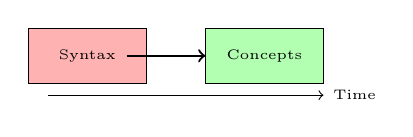
\begin{tikzpicture}[scale=0.5]
          \draw[->] (0,0) -- (7,0) node[right] {\tiny Time};
          \node[draw, rectangle, fill=red!30, minimum width=1.5cm, minimum height=0.7cm, font=\tiny] at (1, 1) {Syntax};
          \node[draw, rectangle, fill=green!30, minimum width=1.5cm, minimum height=0.7cm, font=\tiny] at (5.5, 1) {Concepts};
          \draw[->, thick] (2, 1) -- (4, 1);
        \end{tikzpicture}
      \end{center}
      
      \textbf{What Remains Constant:}
      \begin{itemize}
        \item Execution models
        \item Trade-off reasoning
        \item Debugging skills
        \item API design
      \end{itemize}
    \end{column}
  \end{columns}
  
  \textbf{Key Insight:} Banning LLMs is futile; teaching responsible use is essential.
  
  % Speaker note: Human expertise becomes MORE valuable, not less
\end{frame}
%%%%%%%%%%%%%%%%%%%%
